\Titular%
{\textit{Strike, you're out!} Bombas, Heisenberg e un catcher}%
{Santiago González Gómez}%
{historia}%
{As vidas dun beisbolista e dun dos pais da Física Cuántica, cruzadas por unha
historia de espías e o proxecto atómico da Alemaña nazi.}%

\begin{refsection}
\begin{multicols}{2}

\subsection*{Heisenberg e o \textit{proxecto Uranio}}

Cando en setembro de 1939 estourara a Segunda Guerra Mundial, Werner
Heisenberg, un dos pais da física cuántica, foi requirido polo goberno nazi
xunto con outros destacados físicos alemáns. O estudo da fisión nuclear
atopábase en auxe e Alemaña quería estudar a viabilidade de construír unha
bomba que empregase este novo campo como elemento destrutivo. Comezaba así o
\textit{proxecto Uranio}, o análogo alemán ao \textit{proxecto Manhattan}
estadounidense.

A posición de Heisenberg era delicada. Aínda que se opoñía ao réxime nazi,
tamén era un fervente patriota alemán, e temía que unha derrota de Alemaña na
guerra resultase nunha ocupación soviética de Europa, algo que consideraba
bastante peor que o dominio nazi. Por outra banda, tampouco tiña moita elección
sobre a súa participación no proxecto; non só pola posibilidade de perder o seu
traballo, senón porque a súa relación con científicos xudeus antes da guerra
facíao sospeitoso a ollos de moitos nazis.

\begin{centering}
    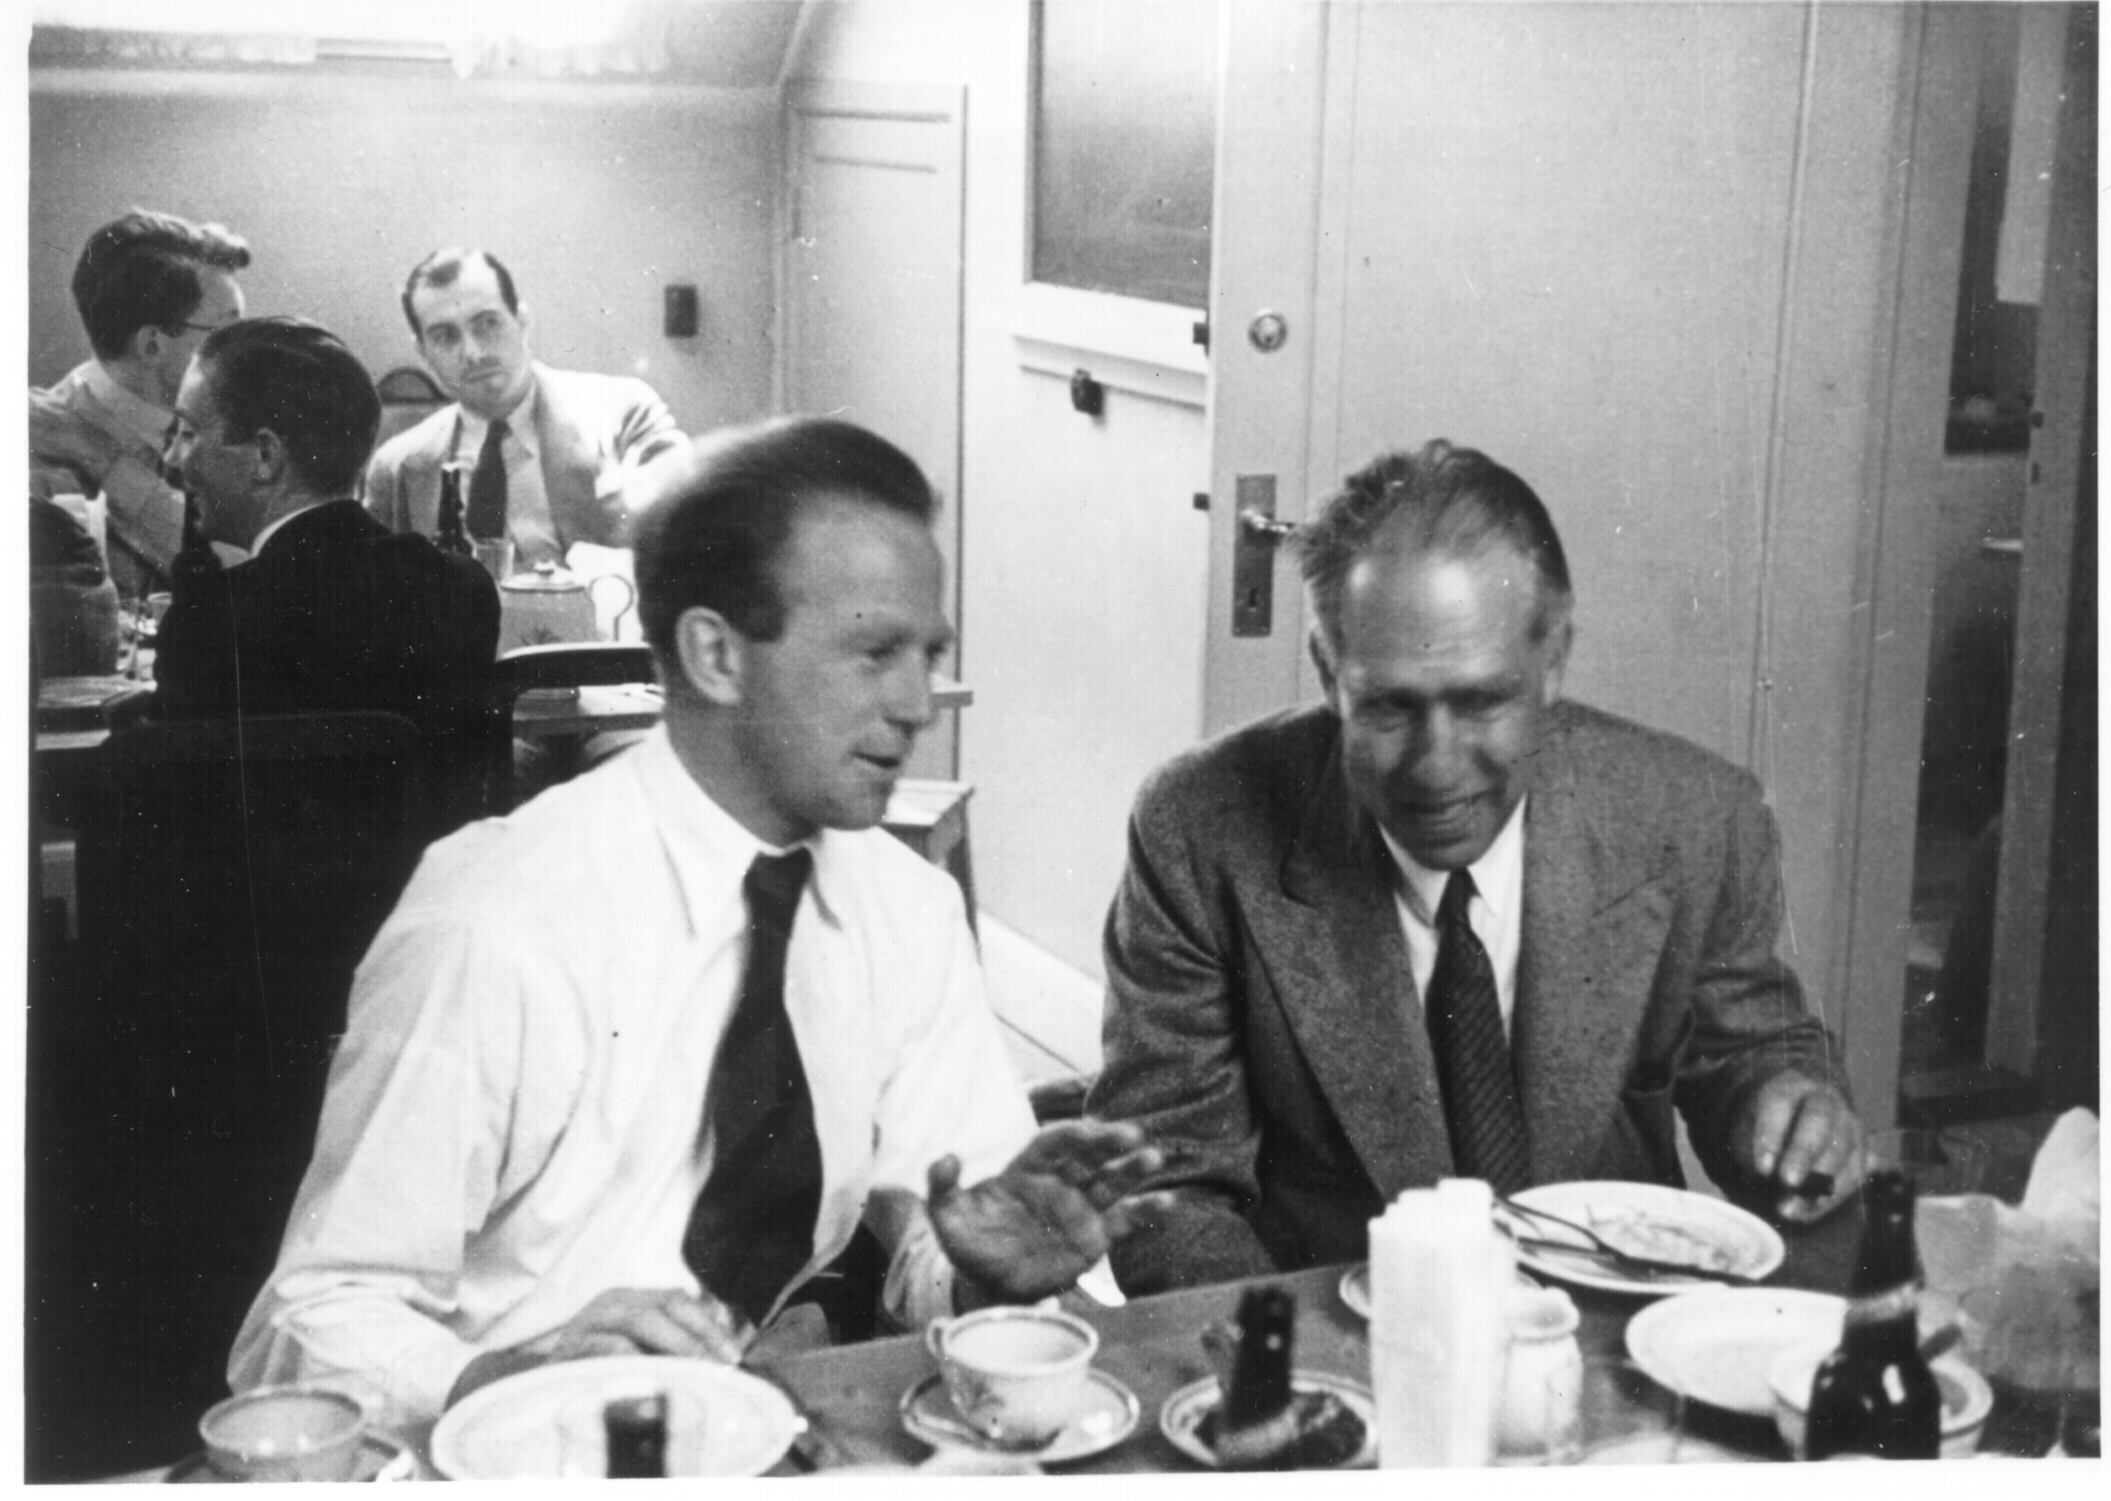
\includegraphics[width=0.65\linewidth]{revistas/002/imaxes/bohr.jpg}
    \captionof{figure}{Heisenberg e Bohr nun encontro en 1941. Fonte: Niels Bohr Archive.}
\end{centering}

Sexa como for, Heisenberg pasara dous anos investigando intensamente ata
concluír, en 1941, que malia ser posible construír a bomba (tanto de uranio
como de plutonio), esta levaría demasiado tempo e consumiría demasiados
recursos alemáns. Heisenberg consideraba ademais que os rivais de Alemaña
chegarían ás mesmas conclusións. Os líderes nazis aceptaron a súa opinión e o
\textit{proxecto Uranio} pasou a investigar a posibilidade de construír un
reactor nuclear que producise enerxía eléctrica.

Para Heisenberg, o posible desenvolvemento dunha bomba nuclear supuña un dilema
moral importante, así que chegar a esta conclusión foi, dende logo, un alivio.
Porén, a idea (ou mellor dito, o medo) de ter que construír unha bomba nuclear
nun futuro nunca abandonou a súa cabeza. Aproveitando unha visita a Dinamarca,
deixou caer ao seu vello mentor Niels Bohr as súas dúbidas morais sobre a
producción de armamento atómico. Bohr creu que Heisenberg lle estaba a tender
algún tipo de trampa deseñada pola Gestapo e preferiu cambiar de tema.

\subsection*{``O home máis intelixente do béisbol''}

Para o ano 1942 e, ao outro lado do Atlántico, os Estados Unidos iniciaban o
seu propio programa atómico: o \textit{proxecto Manhattan}. Pero remontémonos
algo máis atrás no tempo...

En 1934, un equipo de \textit{all-stars} do béisbol estadounidense fixo unha
xira por Xapón, onde o béisbol comezaba a ser un deporte cada vez máis popular.
Xunto a todas as estrelas, viaxou co equipo un \textit{catcher} mediocre, que
levaba anos saltando de equipo a equipo na liga sen destacar especialmente: Moe
Berg. Berg, de orixe xudía, ten sido descrito como ``o beisbolista máis estraño
da historia'' ou ``o home máis intelixente do béisbol''. Aínda que non era un
xogador especialmente destacado, si era tremendamente astuto, e tiña unha
habilidade innata para os idiomas, de aí que estudara a fondo polo menos sete
diferentes. Precisamente, a razón pola que Berg viaxara a Xapón en 1934 era
pola súa capacidade para falar xaponés.

Cando os Estados Unidos entraran na Segunda Guerra Mundial, Berg alistouse e
pasou por varios destinos lonxe da fronte. En 1943, uniuse á OSS, a precursora
da actual CIA, onde fora moi valorada a súa capacidade para os idiomas. Berg
realizou primeiramente varias misións como espía en Iugoslavia, onde
investigaba grupos partisanos que os Estados Unidos consideraba apoiar.

Cara a 1943, Berg comezou a traballar no \textit{proxecto Larson}, unha
operación cuxo obxectivo inicial era reclutar a físicos italianos e levalos aos
Estados Unidos para que colaborasen no \textit{proxecto Manhattan} e outras
misións armamentísticas. Berg acabou por percorrer varios lugares de Europa
entrevistando a físicos, non só para tentar convencelos de que se mudasen aos
Estados Unidos, senón tamén para obter información sobre Heisenberg. Os
estadounidenses sospeitaban que Heisenberg dirixía un proxecto atómico para os
alemáns, e despois de que Bohr, a quen os aliados sacaron de Dinamarca en 1943
e levaron a Reino Unido para que colaborase con eles, comentase as
conversacións que Heisenberg tivera con el en 1941; era indispensable
determinar como de preto estaba o alemán de desenvolver a temida bomba. A OSS
chegou a considerar a posibilidade de secuestralo, pero isto nunca chegou a
suceder.

\begin{centering}
    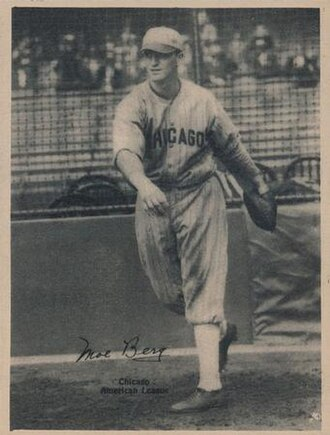
\includegraphics[width=0.55\linewidth]{revistas/002/imaxes/bergChicago.jpg}
    \captionof{figure}{Cromo de Berg mentres xogaba para os Chicago White Sox. Fonte: Wikipedia.}
\end{centering}

En 1944, a OSS soubo que Heisenberg ía dar unha conferencia en Zürich,
territorio neutral. A Berg, que por suposto falaba alemán, asignóuselle a
misión de asistir á dita conferencia e tentar determinar se este estaba preto
de construír a bomba atómica. Se o espía contara coa máis mínima sospeita de
que Heisenberg supoñía un perigo, tiña ordes de levantarse no medio da
conferencia e dispararlle.

Berg non só acudira á conferencia facéndose pasar por estudante de física,
senón que tamén estivo presente nunha festa á que o teórico alemán asistira na
súa estancia en Zürich. O beisbolista saíu do evento á vez que Heisenberg e
entablou diálogo con el no camiño de volta; non houbo nada nestas conversas que
fixese sospeitar a Berg. O patriota alemán admitira durante a festa que a
guerra estaba perdida para os alemáns, algo que Berg xulgou que non diría
alguén que estaba a piques de rematar unha bomba atómica. Tamén reflexionou
que, aínda que tería sentido matar a Heisenberg en 1942 nos inicios dun suposto
proxeto de bomba atómica alemá, para o 1944 xa sería demasiado tarde.
Finalmente, decidiu non asasinar a Heisenberg e as súas vidas separáronse para
non volver a atoparse nunca máis.

\subsection*{Unha granxa en Cambridge}

Moito se ten discutido sobre o papel de Heisenberg no \textit{proxecto Uranio},
considerando que o \textit{proxecto Manhattan} si foi exitoso. De verdade
tentou fabricar a bomba e simplemente non o conseguiu por incompetencia? Ou
saboteou o \textit{proxecto Uranio} por motivos morais, convencendo ao resto
dos seus integrantes da imposibilidade de construír a bomba?

Esta dúbida tamén asaltou aos estadounidenses cando en 1945 capturaron a
Heisenberg e o resto de físicos alemáns do \textit{proxecto Uranio}. Todos eles
foron trasladados á \textit{Farm Hall}, unha mansión campestre inglesa preto de
Cambridge que estaba infesta de micrófonos para espiar as súas conversas. O 6
de agosto, os aliados aseguráronse de que Heisenberg e os demais escoitasen a
transmisión de radio do bombardeo de Hiroshima. Heisenberg inicialmente negouse
a crer que a bomba fose atómica, argumentando que a masa crítica (a masa mínima
de material radioactivo necesario para soster a reacción nuclear) necesaria
para unha bomba desas características debía ser dúas toneladas polo menos,
imposible de fabricar para os estadounidenses. Para decatarse do errado desta
afirmación, nótese que a bomba detonada posteriormente sobre Nagasaki contiña
64 kg de uranio enriquecido.

Que ocorreu? Mentía Heisenberg ao réxime nazi dando un valor falso da masa
crítica para impedir a fabricación da bomba? Non é tan sinxelo. Días despois,
fixo os cálculos e expuxo aos seus compañeiros como cría que os estadounidenses
fabricaran a bomba, estes cálculos resultaron ser moi correctos. Os físicos do
\textit{proxecto Manhattan} concluíron que o alemán simplemente \textit{nunca
antes realizara os cálculos} da masa crítica. Heisenberg estaba moito máis
interesado no desenvolvemento dun reactor que no dunha bomba e, imaxinándose un
valor desorbitado para a masa crítica, simplemente decidiu non facer os
cálculos. Posiblemente prefiría vivir no descoñecemento a afrontar o dilema
moral da construción da bomba.

Dende logo, ás veces é abrumador pensar como as decisións do individuo menos
esperado son capaces de cambiar o rumbo da historia.

\nocite{gottstein.k_2016}
\nocite{dawidoff.n_2011}

\printbibliography

\end{multicols}
\end{refsection}
